\documentclass[10pt,journal,compsoc]{IEEEtran}

\usepackage{ctex}
\usepackage{times}
\usepackage{epsfig}
\usepackage{graphicx}
\usepackage{amsmath}
\usepackage{amssymb}
\usepackage{hyperref}
\usepackage{enumerate}
\usepackage{enumitem}
\usepackage{caption}
\usepackage{color}
\usepackage{comment}
\usepackage{url}
\usepackage{xcolor}
\usepackage{tabu}
\usepackage{booktabs}
\usepackage{makecell}
\usepackage{wrapfig}
\usepackage{breakcites}
\usepackage{subfig}
\usepackage{ragged2e}
\usepackage{stfloats}
\usepackage{xcolor}
\usepackage[export]{adjustbox}
\usepackage{indentfirst}
\setlength{\parindent}{2em} 
\usepackage{stfloats}

\usepackage{amsfonts}       % blackboard math symbols
\usepackage{nicefrac}       % compact symbols for 1/2, etc.
\usepackage{microtype}      % microtypography
\usepackage{lipsum}
\usepackage{adjustbox}
\usepackage{pifont}

\usepackage{multirow}

\usepackage{algorithm}
\usepackage[noend]{algpseudocode}

% 定义代码样式
\usepackage{listings}

\definecolor{gray}{rgb}{0.96,0.96,0.96}

\lstset{ %
  language=python,                % the language of the code
  basicstyle=\footnotesize,           % the size of the fonts that are used for the code
  numbers=left,                   % where to put the line-numbers
  columns=fixed, 
  numberstyle=\tiny\color{black},  % the style that is used for the line-numbers
  stepnumber=1,                   % the step between two line-numbers. If it's 1, each line 
                                  % will be numbered
  numbersep=1.5mm,                  % how far the line-numbers are from the code
  xleftmargin=1.3em,
  backgroundcolor=\color{gray},      % choose the background color. You must add \RequirePackage{color}
  showspaces=false,               % show spaces adding particular underscores
  showstringspaces=false,         % underline spaces within strings
  showtabs=false,                 % show tabs within strings adding particular underscores
  frame=single,,                 % adds a frame around the code
  frameround = tttt,
  framexleftmargin=3mm, 
  rulecolor=\color[RGB]{158,193,243},        % if not set, the frame-color may be changed on line-breaks within not-black text (e.g. commens (green here))
%  aboveskip=1em,
  tabsize=2,                      % sets default tabsize to 2 spaces
  captionpos=b,                   % sets the caption-position to bottom
  breaklines=true,                % sets automatic line breaking
  extendedchars=false,   
  breakatwhitespace=false,        % sets if automatic breaks should only happen at whitespace
  title=\lstname,                   % show the filename of files included with \lstinputlisting;
                                  % also try caption instead of title
  keywordstyle=\color[RGB]{0,51,179},          % keyword style
  commentstyle=\color[RGB]{140,140,140},       % comment style
  stringstyle=\color[RGB]{6,125,23},         % string literal style
  identifierstyle=\color{black},
  escapeinside={\%*}{*)},            % if you want to add LaTeX within your code
  morekeywords={*,...}               % if you want to add more keywords to the set
}

\def\Plus{\texttt{+}}

\makeatletter
\def\BState{\State\hskip-\ALG@thistlm}
\makeatother

\graphicspath{{figures/}}

% *** CITATION PACKAGES ***
%
\ifCLASSOPTIONcompsoc
  % IEEE Computer Society needs nocompress option
  % requires cite.sty v4.0 or later (November 2003)
  \usepackage[nocompress]{cite}
\else
  % normal IEEE
  \usepackage{cite}
\fi

% *** GRAPHICS RELATED PACKAGES ***
%
\ifCLASSINFOpdf

\else

\fi

\hyphenation{op-tical net-works semi-conduc-tor}


\begin{document}
\begin{sloppypar}

\title{数字图像处理:前沿技术}

\author{唐麒\qquad 21120299\\qitang@bjtu.edu.cn}

\IEEEtitleabstractindextext{
\begin{abstract}
\justifying 对齐向来是视频超分辨率重建(Video Super-Resilution, VSR)中的重要操作,然而自注意机制的进展可能会违背这一常识。本文重新思考了 Transformer VSR 中对齐的作用,并进行了一些反直觉的观察。实验表明,VSR Transformer 可以直接使用未对齐的多帧信息,而现有的对齐方法可能并不适用 VSR Transformer。此外,简单的移除对齐模块并采用更大的注意窗口可以进一步提高  VSR Transformer 的性能。然而,这种设计将大大增加计算负担,并不能处理大的运动。为此,本文提出了一种基于 patch 的对齐方法,该方法利用图像 patch 代替像素进行对齐并获得 SOTA 表现。

\end{abstract}

\begin{IEEEkeywords}
视频超分辨率重建、Transformer、光流
\end{IEEEkeywords}}


% make the title area
%\maketitle

\twocolumn[{%
\renewcommand\twocolumn[1][]{#1}%
\maketitle
\pagenumbering{arabic}

\vspace{-1.5cm}
\noindent\begin{minipage}{\linewidth} 
 	\begin{center}
 	\captionsetup{font=small}
 	\begin{tabular}{@{}c@{}c@{}c@{}}
% 	\includegraphics[width=0.31\linewidth,cframe=red!50!black 1mm]{fig1_a} &
% 	\includegraphics[width=0.31\linewidth,cframe=green!50!black 1mm]{fig1_b} &
%    \includegraphics[width=0.313\linewidth,cframe=blue!50!black 1mm]{fig1_c} \vspace{-1mm}\\
	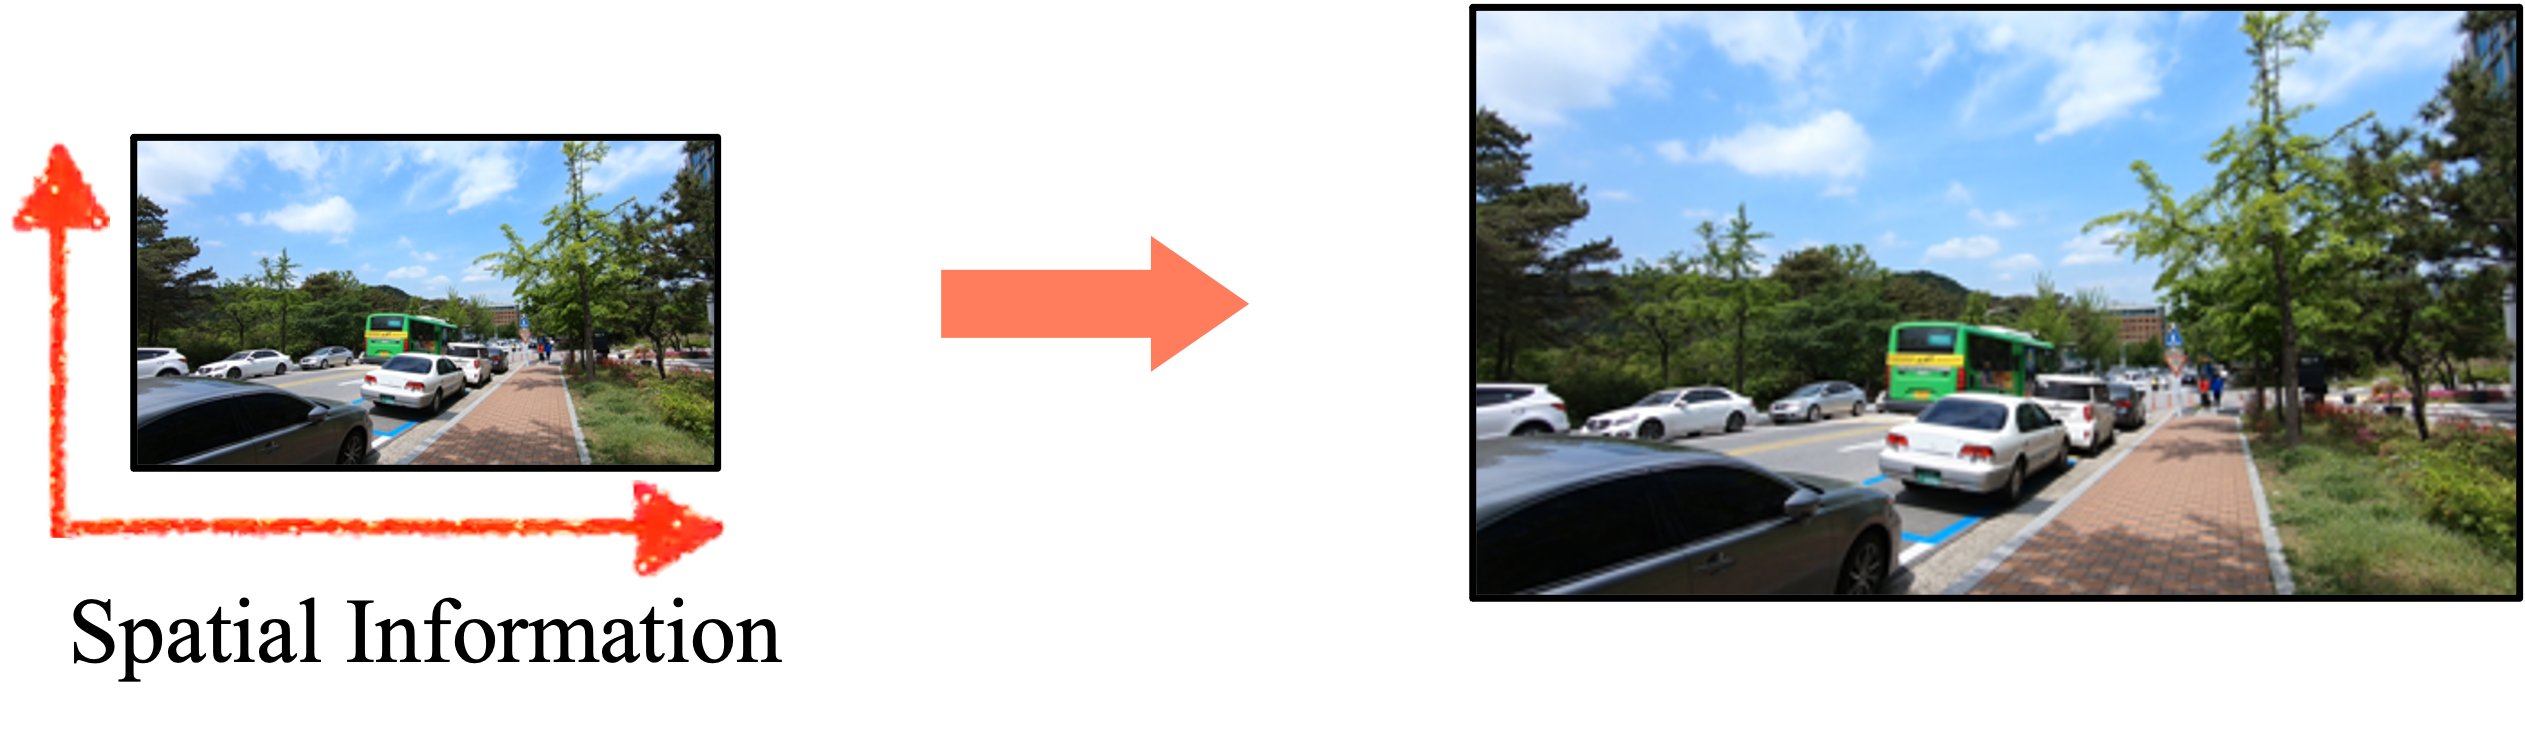
\includegraphics[width=0.48\linewidth]{1} &
    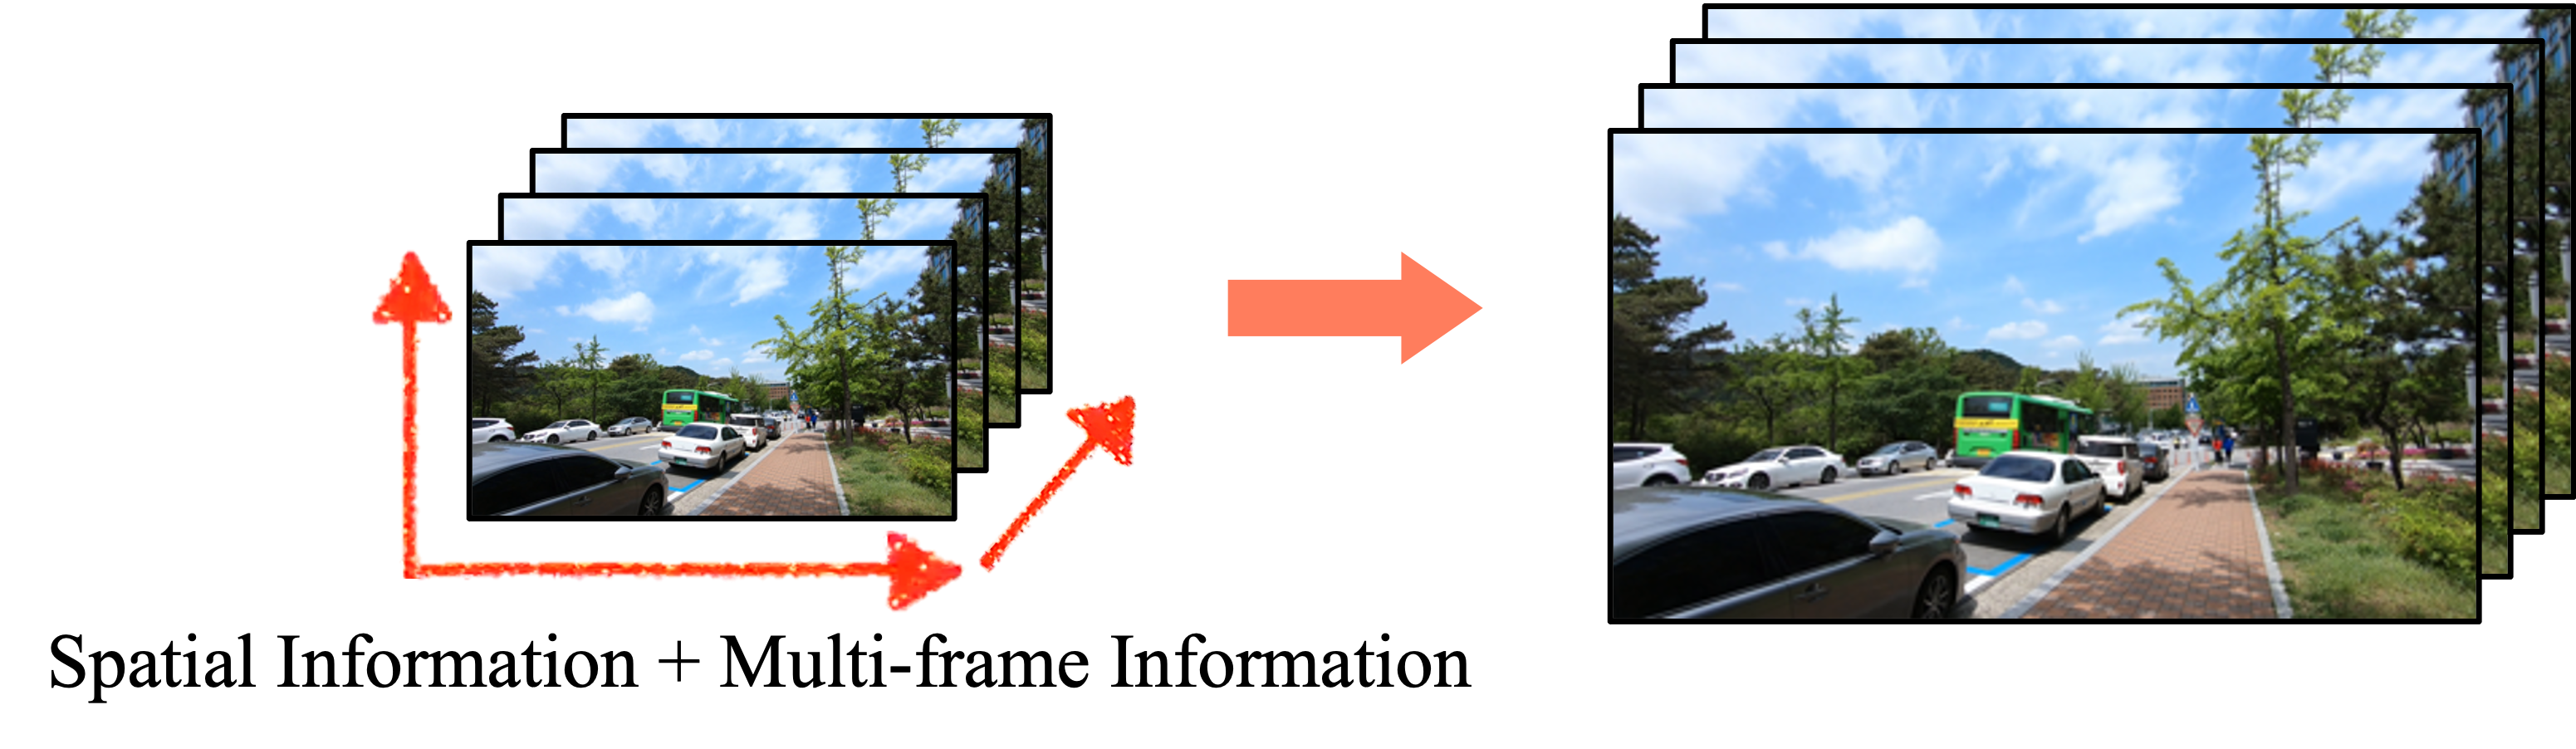
\includegraphics[width=0.48\linewidth]{2}\\
    {\small (a)} &  {\small (b)}  \\
    \end{tabular}
	\captionof{figure}{\small 超分辨率重建任务示意图: (a) 图像超分辨率重建, (b) 视频超分辨率重建}
	\label{fig:random_thresholding}
	\end{center}  \vspace{1.25cm}
\end{minipage}
}]

\IEEEraisesectionheading{\section{简介}
\label{sec:introduction}}

超分辨率重建指的是将给定的低分辨率图像恢复成相应的高分辨率图像,单图超分旨在利用空间信息将给定的低分辨率图像恢复成相应的高分辨率图像,而对于视频来讲,多帧高度相关但不对齐的图像可以为超分提供更加丰富的信息,对这些帧间信息的利用是几乎所有视频恢复任务比较核心的研究课题。

如 \textbf{图 \ref{fig:fig2}} 所示,可以看到对孔洞进行恢复时,单图超分由于难以获得语义信息,所以恢复得不太准确,而视频超分由于综合了多帧的信息,可以恢复出更加准确的细节。而在日常拍照时,快门按下去并不一定是一帧被采集,而是会连续采集很多帧,帧之间微小的抖动可以提供了很多视频恢复使用的亚像素信息。


上面一排是相同的但有微小位移的高分辨率图片,下面是对应的低分辨率版本。虽然都占据了相同的像素,但是当高分辨率的图像位移1/4或者1/2个像素的时候,产生的低分辨率的版本是不同的,由位移产生的这些不同模式就是所说的亚像素的信息。

上面一排是有微小位移的相同高分辨率图片,下面是对应的低分辨率版本。虽然都占据了相同的像素,但是当高分辨率图像位移1/4或者1/2个像素的时候,产生的低分辨率的版本是不同的,由位移产生的这些不同模式就是所说的亚像素的信息。

对于单图和视频超分,一个朴素的做法就是使用相同的超分网络,单图把所有的空间信息交给网络去预测,对于视频可以把帧间的信息叠在一起之后交给网络预测。但有一个问题就是视频里面的物体是会移动的,而由于 CNN 具有局部性的归纳偏置,这显然是行不通的。因此需要对网络进行一些特殊的模块设计。

\begin{figure}[!tbp]
	\centering
	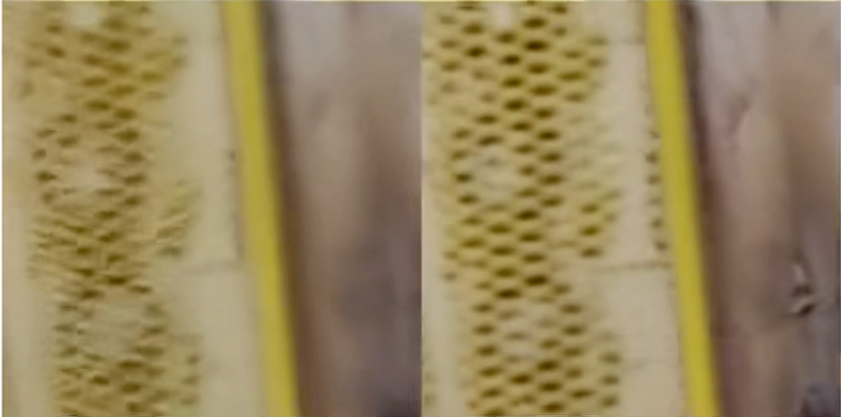
\includegraphics[width=0.9\linewidth]{3.png}
	\caption{SISR 和 VSR 模型的视频超分辨率重建结果:左:SISR, 右:VSR}
	\label{fig:fig2}
\end{figure}
\section{相关工作}
\label{sec:related_work}

\begin{figure*}
	\centering
	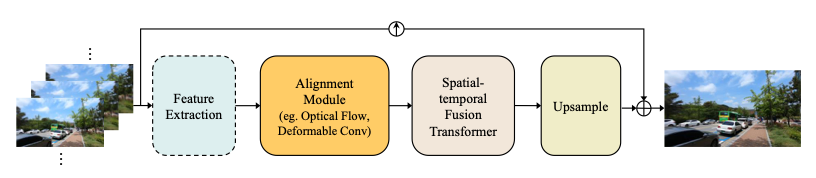
\includegraphics[width=\linewidth]{6.png}
	\caption{VSR 网络模块示意图}
	\label{fig:fig6}
\end{figure*}

\begin{table*}[!t]
\caption{Components in existing VSR methods. }
	\begin{center}
		\tabcolsep=0.1cm
		\scalebox{0.9}{
			\begin{tabular}{l|c|c|c|c|c|c|c|c}
				\hline
				\multirow{2}{*}{} & \multicolumn{3}{c|}{Sliding-Window} & \multicolumn{5}{c}{Recurrent}                                                                                                                                                                                                            \\ \cline{2-9}
				%
				                  & EDVR      & MuCAN      & TDAN & BRCN & FRVSR  & RSDN  & \textbf{\mbox{BasicVSR}} & \textbf{\mbox{IconVSR}}          \\ \hline
				%
				Propagation       & Local                               & Local                         & Local                    & \textbf{Bidirectional}                            & Unidirectional                & Unidirectional              & \textbf{Bidirectional}   & \textbf{Bidirectional} (coupled) \\
				Alignment         & \textbf{Yes} (DCN)                  & \textbf{Yes} (correlation)    & \textbf{Yes} (DCN)       & No                                                & \textbf{Yes} (flow)           & No                          & \textbf{Yes} (flow)      & \textbf{Yes} (flow)              \\
				Aggregation       & Concatenate + \textbf{TSA}          & Concatenate                   & Concatenate              & Concatenate                                       & Concatenate                   & Concatenate                 & Concatenate              & Concatenate + \textbf{Refill}    \\
				Upsampling        & Pixel-Shuffle                       & Pixel-Shuffle                 & Pixel-Shuffle            & Pixel-Shuffle                                     & Pixel-Shuffle                 & Pixel-Shuffle               & Pixel-Shuffle            & Pixel-Shuffle                    \\ \hline
			\end{tabular}}
		\vspace{-0.3cm}
	\end{center}
\end{table*}

\begin{figure}[!htbp]
\vspace{-5mm}
  \centering
  \begin{minipage}[b]{\linewidth} 
    \subfloat[]{
    \begin{minipage}[b]{0.25\linewidth}
      \centering
      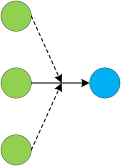
\includegraphics[width=\linewidth]{5-1.png}
     \end{minipage}
  }
  \hspace{5mm}
   \subfloat[]{
    \begin{minipage}[b]{0.25\linewidth}
      \centering
      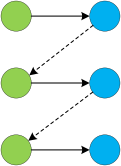
\includegraphics[width=\linewidth]{5-2.png}
     \end{minipage}
  }
   \hspace{5mm}
  \subfloat[]{
    \begin{minipage}[b]{0.25\linewidth}
      \centering
      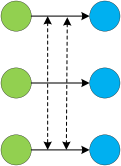
\includegraphics[width=\linewidth]{5-3.png}
     \end{minipage}
  }
      \end{minipage}
  \caption{VSR 网络架构示意图:(a) Sliding-Window;(b) Recurrent;(c) Transformer}
  \label{fig:fig5}
\end{figure}

在 BasicVSR 中,作者将 VSR 网络分为4个功能块 Propagation、Alignment、Aggregation(Fusion)、Upsampling,如 \textbf{图 \ref{fig:fig6}} 所示,针对 VSR 的网络设计也主要是从这四个方面入手。如 \textbf{图 \ref{fig:fig5}} 所示,根据 VSR 利用视频序列信息的方式,可以将现有网络分为Sliding-Window和Recurrent两类。而近期一些工作受 Transformer 模型对序列数据并行计算能力的驱动,将该模型引入到了 VSR 任务中。本文研究的出发点就在于 Transformer 模型对齐模块的设计。

局部性归的纳偏置指的是 CNN 只能看到当前和附近的位置,如 \textbf{图 \ref{fig:fig7}},在 $T_1$ 帧的时候,物体还在画面的右上角,但是到了 $T_2$ 它就往左下角移动了,如果直接将两帧叠在一起输入 CNN,网络根本没有办法利用到 $T_2$ 帧的信息。而在网络中引入 Alignment后,网络会把不同帧的物体挪到相同位置,使得网络可以在一个卷积核里面看到同一个物体在两帧里面的两个版本。

Alignment 基本上是之前所有 VSR 网络必备的模块。自 ViT 之后,Transformer 席卷了整个计算机视觉领域,2021年之后几个效果非常好的 SISR 方法基本上都是基于Transformer的。Transformer 有这么几个特性,例如把输入信号看作离散的token,使用多头自注意力在不同的token之间进行交互等,这些特性使得它非常适合拿来做长程依赖关系的建模。

\begin{figure}[!tbp]
\centering
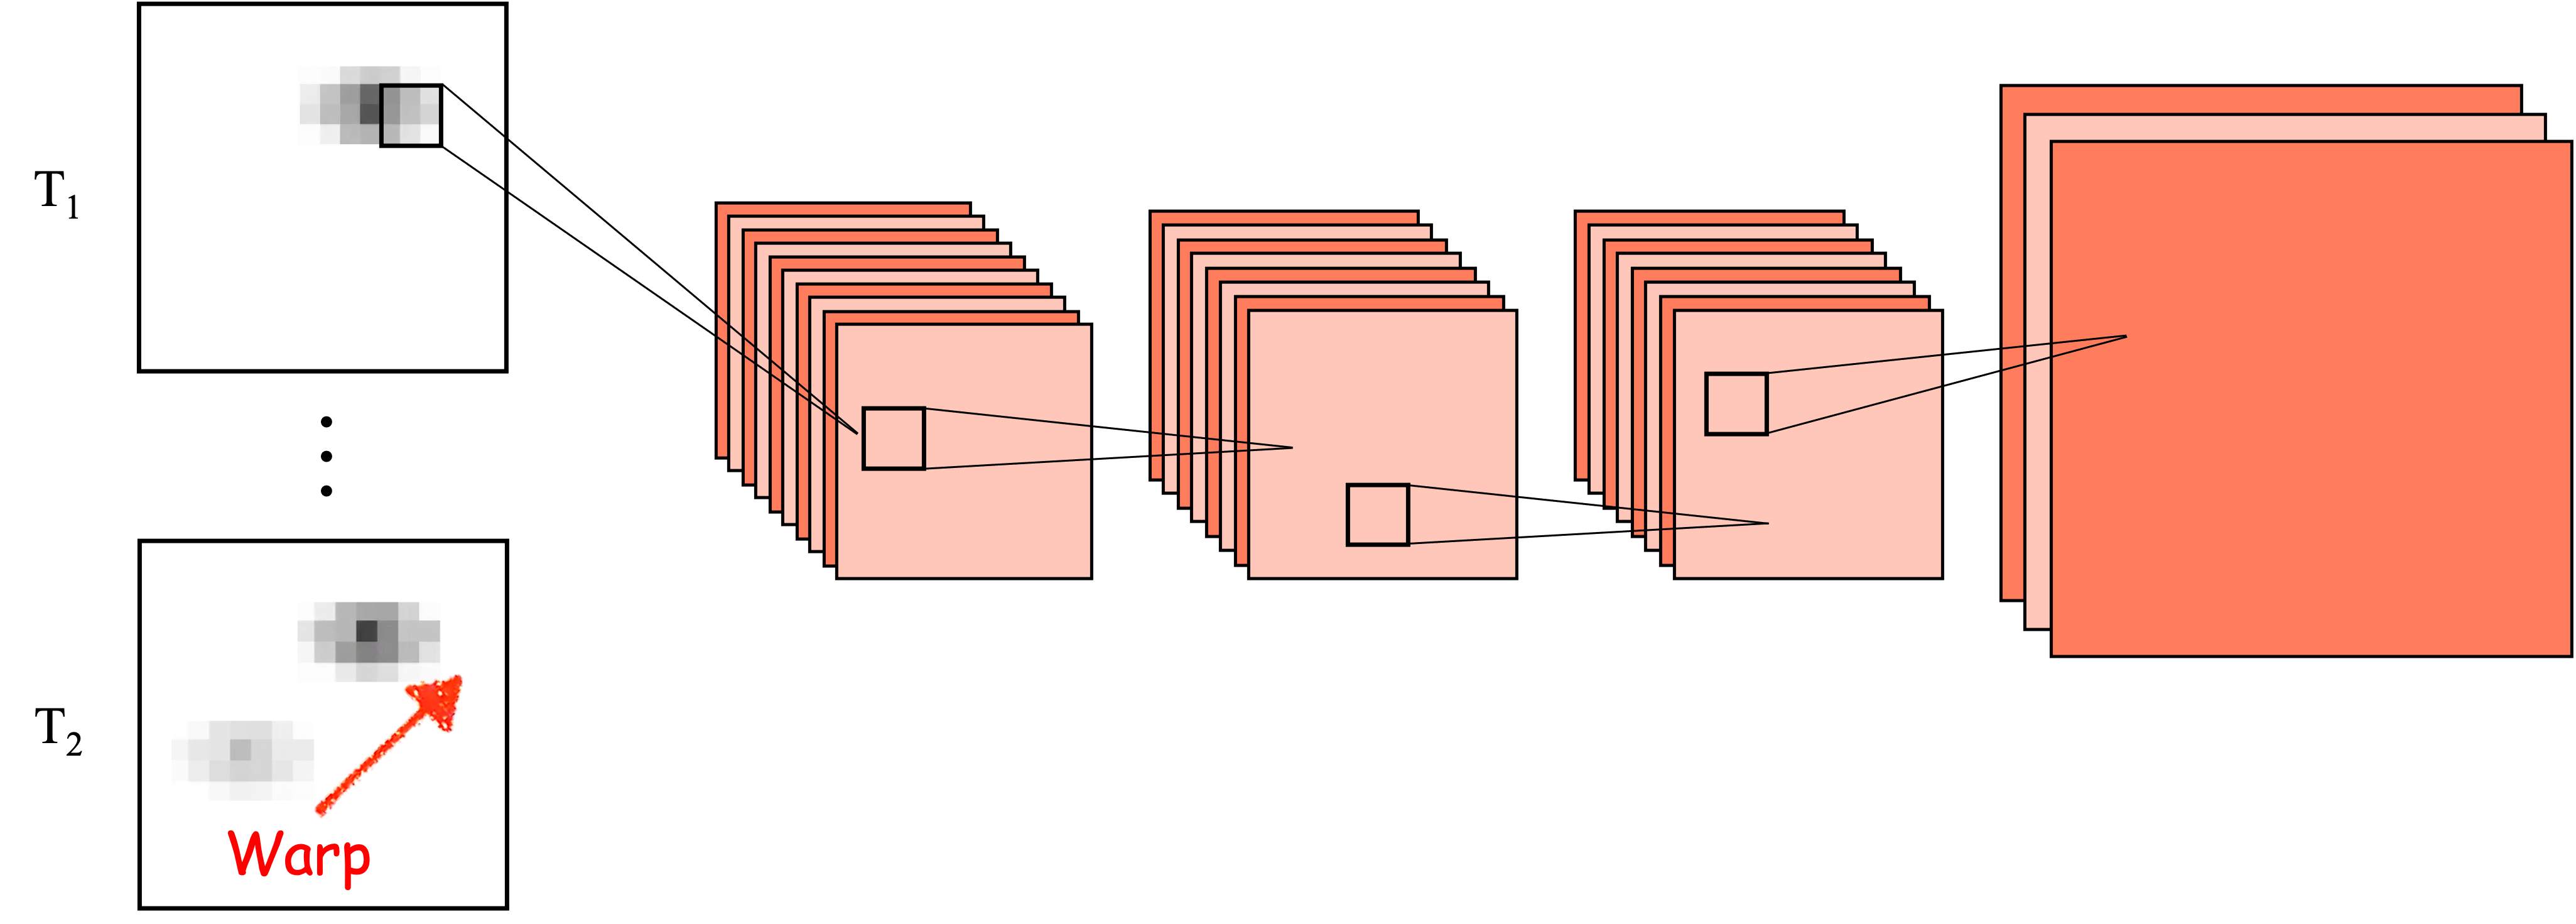
\includegraphics[width=\linewidth]{7.png}	
\caption{卷积神经网络的局部归纳偏置}
\label{fig:fig7}
\end{figure}

第一个特性就是它不像 CNN 是使用卷积或者滤波器去处理相邻两个像素或者甚至是更多像素之间的关系,Transformer 实际上是把输入信号看作一个一个离散的 token,然后他对空间上的交互或者说元素之间的交互是在token之间进行。在图像处理中,已经有很多工作表明比较高效的方法是把每一个像素都当做一个token。Transformer利用自注意力或者多头自注意力在不同的像素token之间进行交互。自注意力的特性是它非常适合拿来做长程的依赖关系或者分布关系的建模。如 \textbf{图 \ref{fig:fig8}} 所示,绿色的像素和红色的像素距离比较接近,但是绿色像素和蓝色像素离得比较远,在Transformer中,自注意力对他们的计算是一样的,也就是说绿色和红色的计算和绿色和蓝色这两套计算都服从同一套权重的计算方法。所以说对于Transformer来说,它处理绿色和红色和它处理绿色和蓝色没有任何的不同,虽然空间上二者关系并不一样,但是它去处理起来是没有区别的,即图中的两个箭头实际上是等价的。

\begin{figure}[!htbp]
\centering
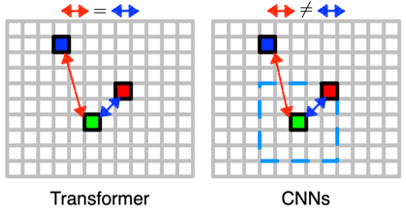
\includegraphics[width=\linewidth]{8.png}	
\caption{卷积神经网络和 Transformer 像素交互示意图}
\label{fig:fig8}
\end{figure}

但是 CNN 就不太一样了,以感受野为 $5 \times 5$ 的卷积为例,对于以绿色像素为中心的卷积操作,红色的像素是在卷积操作的感受野里,所以绿色像素和红色像素是可以在同一层直接进行交互的。但是蓝色的像素并不在这个卷积操作的感受野里面,要是使得绿色的像素和蓝色的像素进行交互,可能要经过多个 CNN 的卷积层,卷积操作的感受野才能作用到那边。此外,即使二者可以在同一个卷积操作的感受野中进行交互,其作用的强度和方法也是不一样的。

CNN 的感受野虽然有那么大,但是并不是感受野里面所有的元素都有同样的权重。越靠近中心的位置,它的权重越大,也就是网络对这个信息利用得越好,而越远离网络对信息利用的越不好。这就是为什么 CNN 会有一个局部性的归纳偏置。而对于视频超分辨率重建而言,只要这个物体挪开了,而且当挪得越远时,网络对信息的利用就越不好。

\begin{figure*}[!hb]
	\centering
	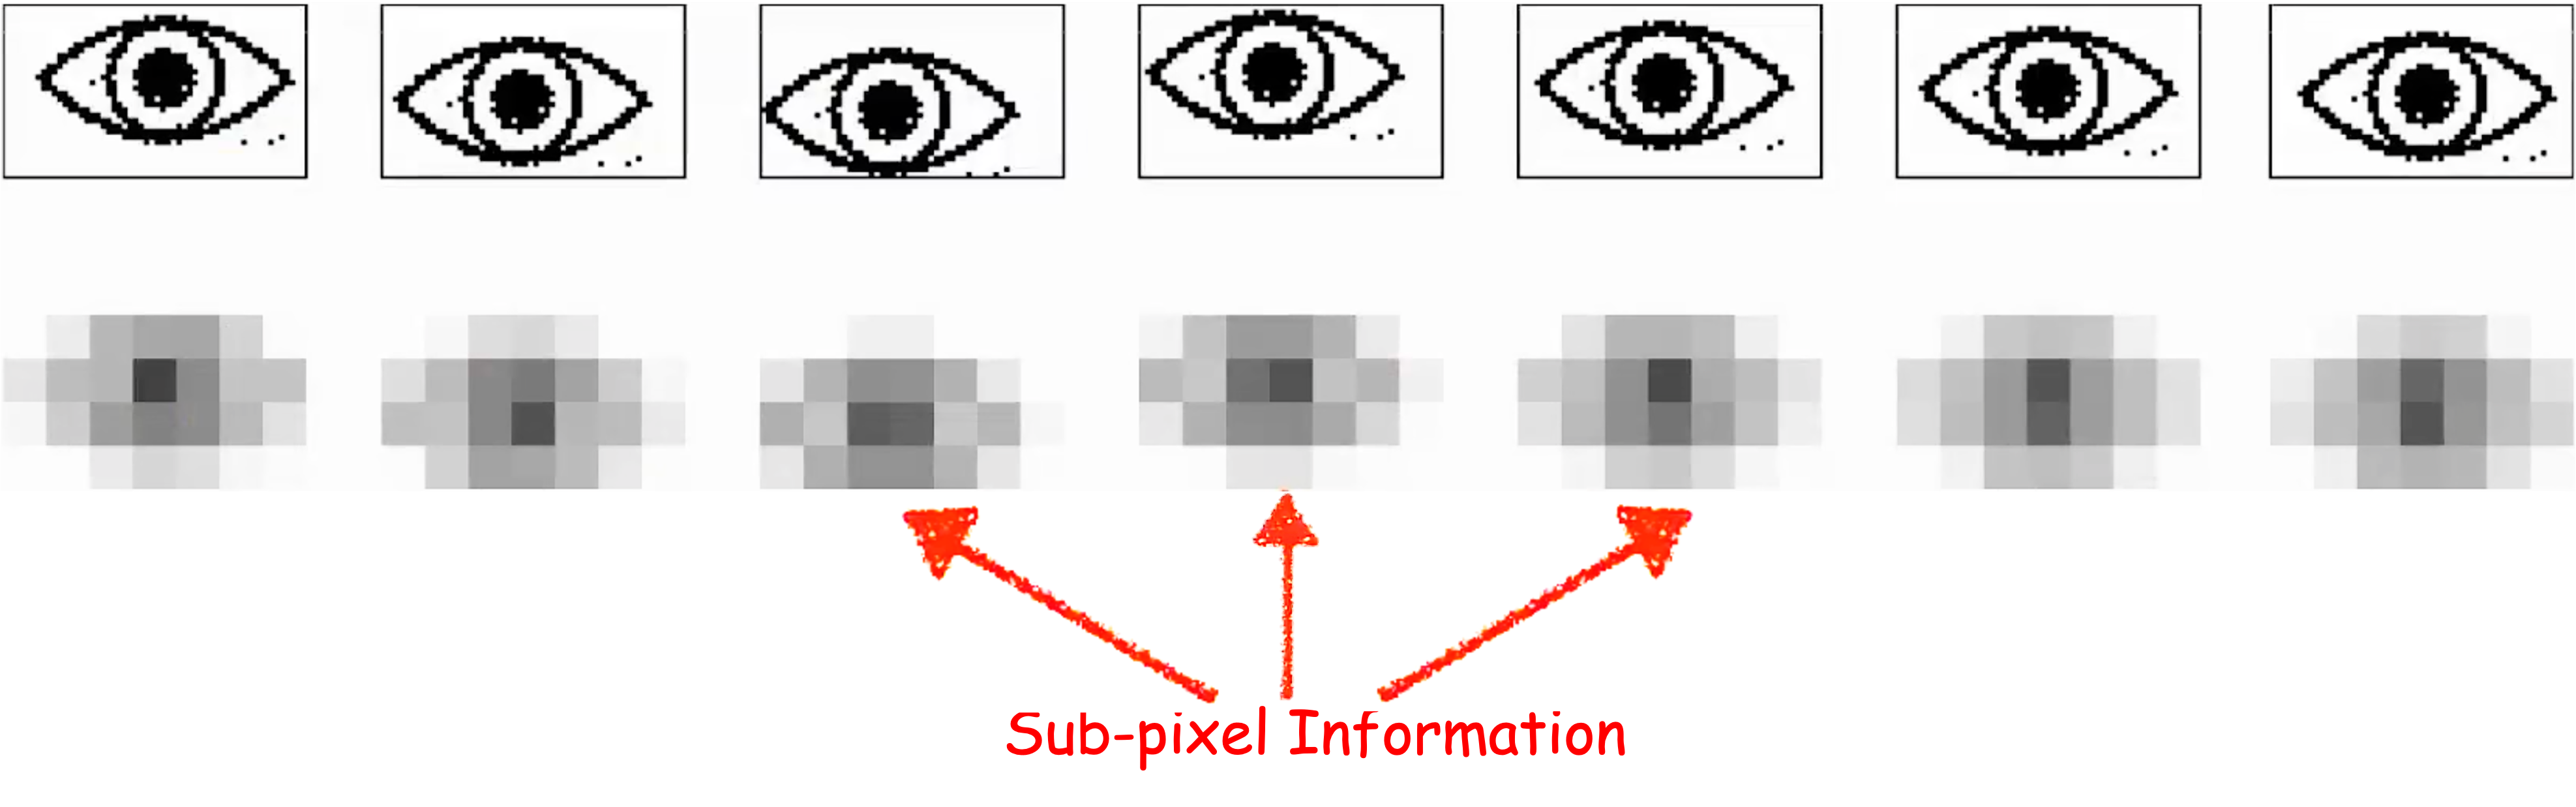
\includegraphics[width=\linewidth]{4.png}
	\caption{亚像素信息示意图}
	\label{fig:fig3}
\end{figure*}

同样,近年来 Transformer 在 VSR 领域的研究也发展迅速。例如减少模型的参数量、在频率域消除压缩伪影的影响等。

\section{方法} 
\label{sec:proposed}

\begin{figure*}[!tbp]
	\centering
	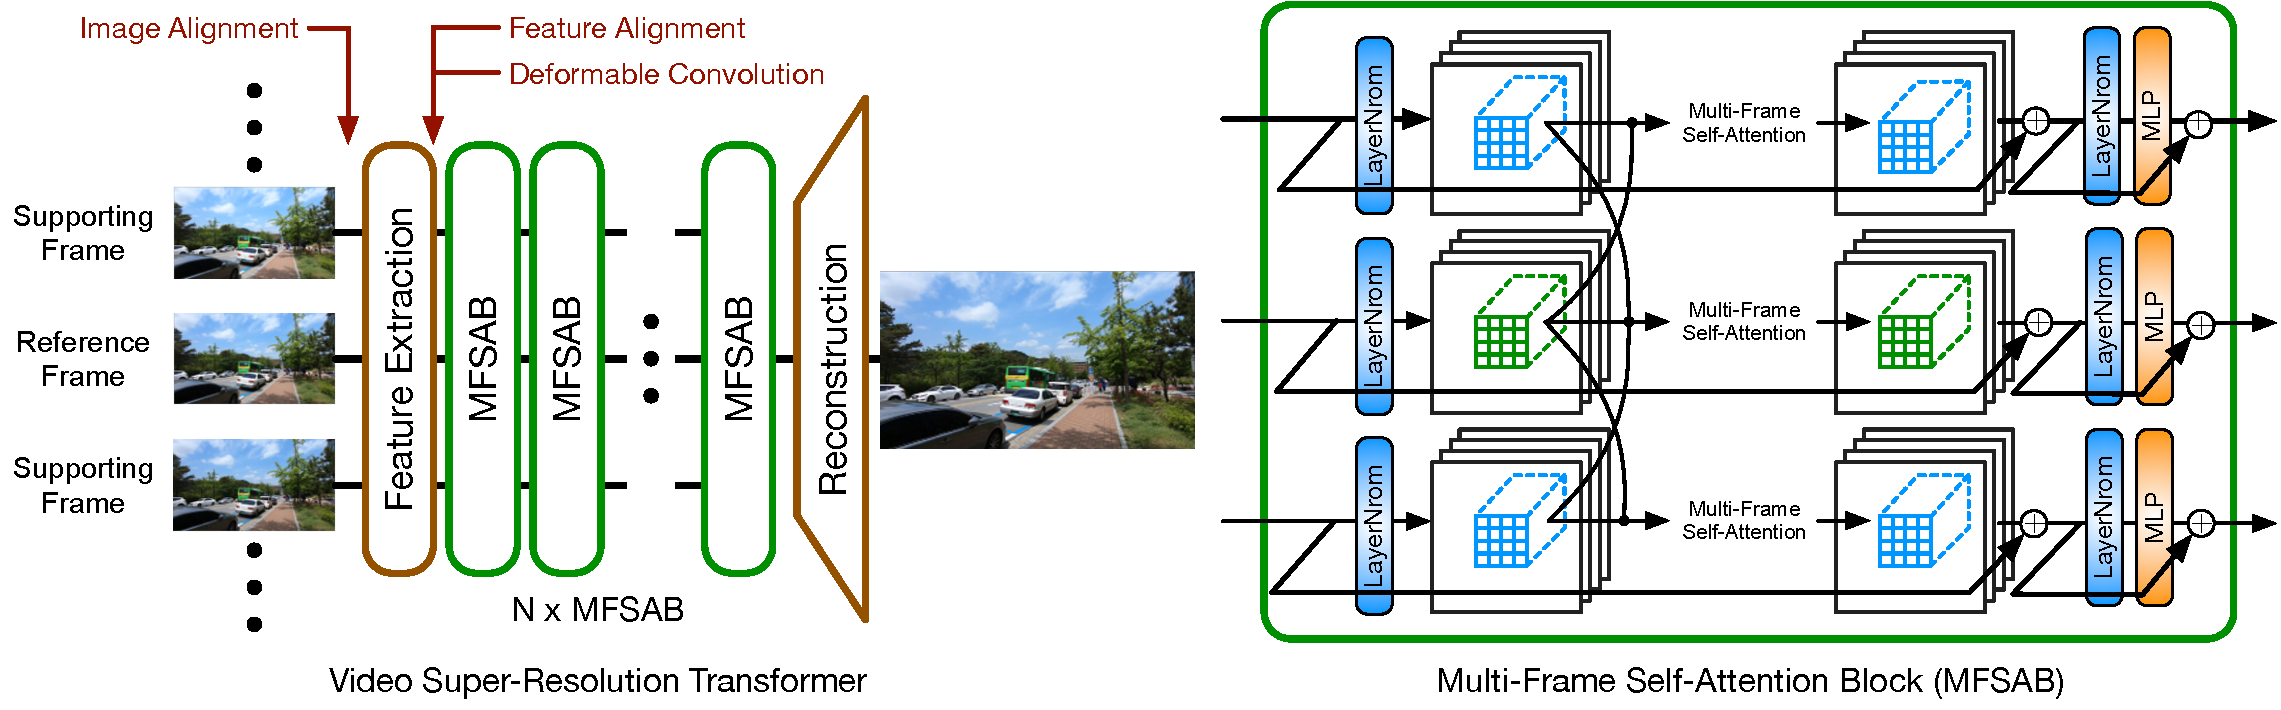
\includegraphics[width=\linewidth]{9.pdf}
	\caption{VSR Transformer 结构示意图}
	\label{fig:fig9}
\end{figure*}

视频超分辨需要 Alignment 是由于 CNN 有非常严格的局部性的归纳偏置而不得不用,但Transformer没有归纳偏置,所以本文提出的第一个思考就是建立一个 VSR 的Transformer 是否仍然需要 Alignment。现有的大部分做法还是延续设计非常复杂的对齐方法,有的时候会占到整个网络近一半的参数。那么自然就会想到如果真的可以不用 alignment,那是用的好还是不用更好呢。

为了研究这两个问题,就需要把这个研究对象给收集起来。使用现有的最基本的图像超分辨或者视频超分辨的Transformer设计来构造了本文的Transformer,如 \textbf{图 \ref{fig:fig9}} 所示,它没有任何特殊的设计。这个模型是基于滑动窗口的,即以三帧作为输入,对中间帧进行超分,前后的这两帧为支持帧(supporting frame),它提供了一些亚像素的信息来支持对中间帧的超分。

Transformer 使用了一个比较通行的标准,即Swin Transformer。Transformer中自注意力的操作会把图像划分成一个一个的局部块。如果不划分局部块而对全局做自注意力的话,在把每一个像素当做一个token的情况下,token数目将会非常多。图像的尺寸增加一倍,token的数量将会增加四倍,其复杂度至少是以 $n^2$ 来增长的。当把图像划分成一个一个的 patch 的时候,即使增大图像的尺寸,其实是patch 的数量在增大,而每一个 patch 里面做的计算仍然是固定数量的像素之间的自注意力操作,其复杂度增加就是线性的。这个 patch 被称为 Attention Window。在这个窗口里面,所有的像素彼此之间有交互,但是窗口和窗口外的像素就没有交互,为了让更多的像素彼此交互,模型会在每一层之间把Attention Window进行位移,称之为 Shift Window。通过这样的方式,就可以让整张图片的任意两个像素可以做一个间接的交互。

本文的模块把 Swin Transformer 从单帧扩展到了一个多帧的情况。例如,原来只有一帧的时候,只是当前 Window $8 \times 8$ 的区域里面 64个像素彼此做自注意力计算。而当把前后帧的像素也纳入进来后,那么同一个位置就是 $3\times 64$(以3帧为例)个像素彼此之间做自注意力计算。

为了研究 Alignment 的影响,还需要对这一模块进行设计。现有的Alignment大致可以分为以下几类:
\begin{enumerate}
	\item 图像对齐是最早最直观的对齐方法。图像对齐依赖于显式计算的帧间光流。根据估计的帧间运动,通过扭曲操作对不同的帧进行对齐。本文使用 SpyNet 来估计光流,并在训练过程中同时对 SpyNet 进行微调,采用 BI 作为重采样方法。
	\item 特征对齐 也可以估计光流,但是是对深度特征进行扭曲操作而不是图像。流估计模块仍然使用SpyNet,在训练时进行优化。除了上图中的二维卷积,此处还额外添加了5个残差块来提取深度特征。
	\item Flow Guide Deformable Convolution 采用可学习的动态可变形卷积进行对齐。几乎所有最先进的VSR网络都使用可变形卷积来进行对齐。本文以 BasicVSR++ 和 VRT 中使用的流引导变形卷积 (FGDC) 对齐作为代表方法。
	\item 无对齐 原始输入直接使用 VSR Transformer 进行处理。
\end{enumerate}


实验涉及到两个主要的Benchmark,一个是REDS,每个视频序列都是比较长的,有100多帧,它的测试集就是REDS 4,有四个100帧左右的测试视频序列。第二个Benchmark的训练集是用Vimeo 90 K,有64,612个训练的视频序列,但是它的每一个视频序列只有七帧。它的测试集有两个数据集,第一个就是Vimeo 90 K的测试集,有7,824 个也是七帧的视频序列,另外一个就是Vid4 测试集。

\begin{figure}[!tbp]
\centering
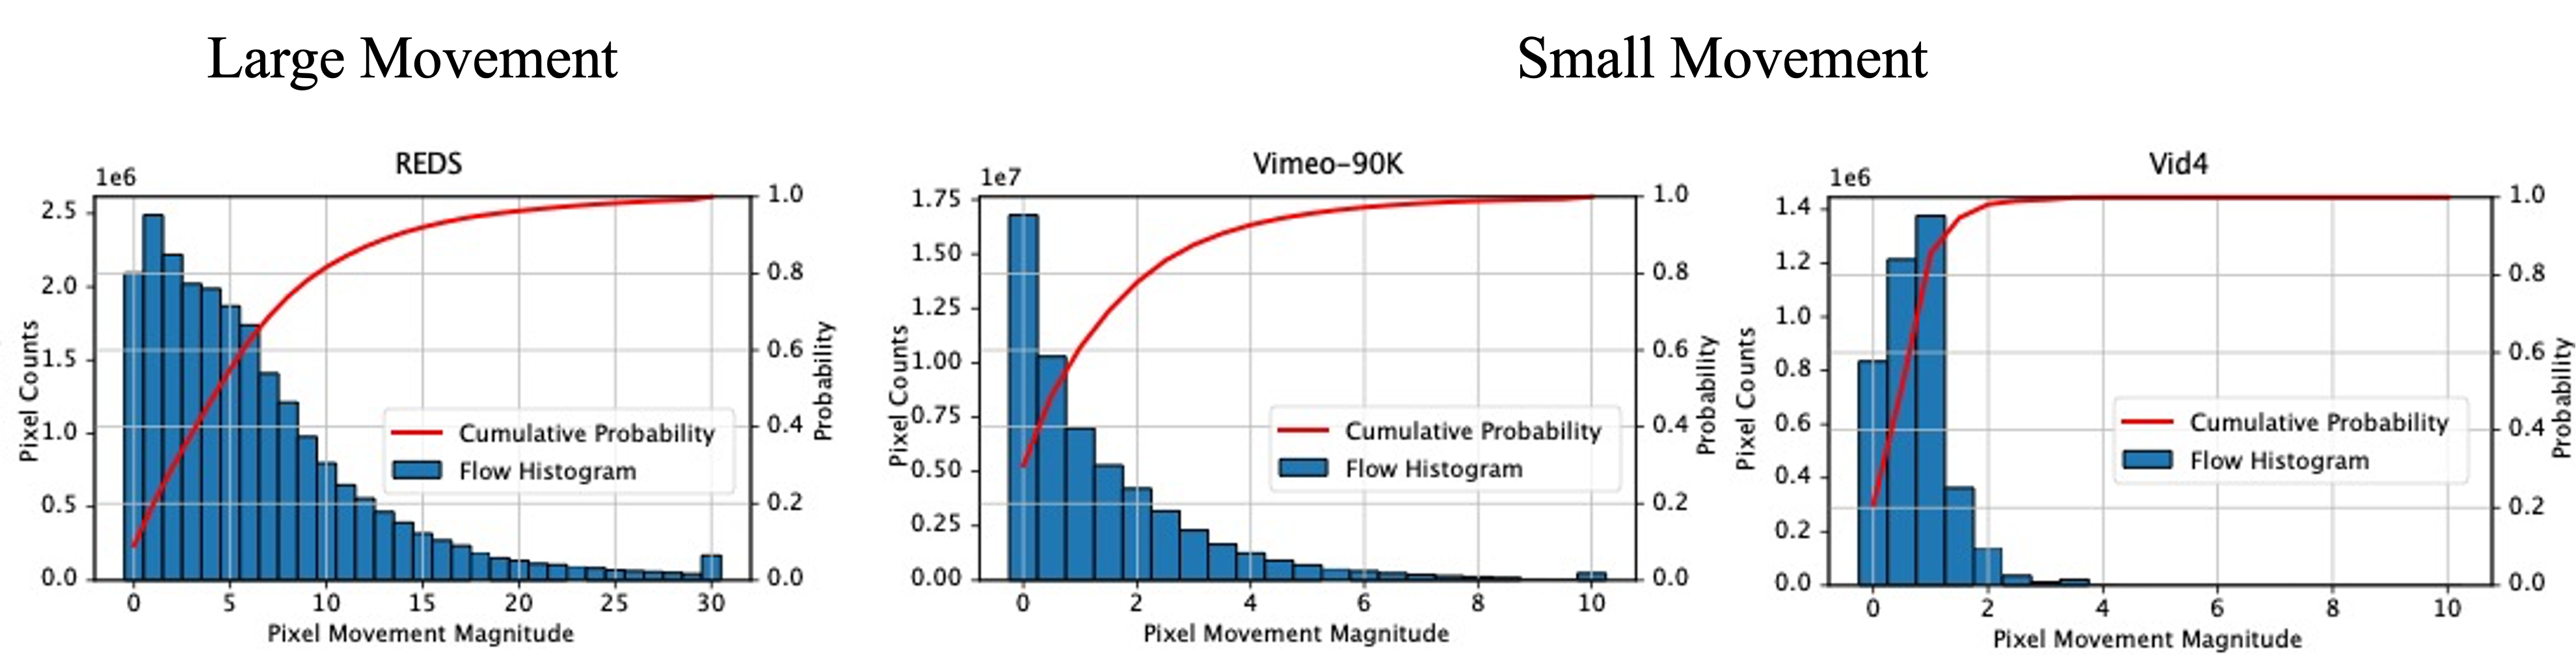
\includegraphics[width=\linewidth]{10.png}	
\caption{不同像素移动条件下,w/o Alignment的VSR Transformer的性能差异}
\label{fig:fig10}
\end{figure}


如 \textbf{图 \ref{fig:fig10}} 所示,可以看到左边的是对 READS 数据集运动情况的统计,在两帧之间,有非常多的物体
是移动了10个、20个甚至30个像素,它的运动来说相对来说非常大。但是右边的这两个数据集,连超过四个像素的运动都非常的少。

回答第一个问题,是不是还要在Video Super-Resolution Transformer里面使用 Alignment的操作呢。

第一个实验使用同一套Transformer的架构构建了两个模型,一个模型使用的是Image Alignment,即先使用光流把图像进行对齐之后再输入到Transformer里面,第二个是不使用Alignment直接输入模型。然后对比不同运动情况像素的 PSNR,如 \textbf{图 \ref{fig:fig11}} 所示,图中大于零的部分代表的是不使用 Alignment会更好,小于零的部分呢是代表使用Alignment会更好。红色的线呢是代表位移是八个像素的这么一条线。在位移小于八个像素的时候,不使用 Alignment明显更好,但是大于八个像素之后,必须使用Alignment才能取得一个更好的成绩。这个八正是Transformer的注意力窗口大小。这个结果表明这个Transformer其实也不是严格意义上的没有归纳偏置,当两个像素同时出现在同一个Window里面时,它可以彼此之间进行直接的交互,不使用Alignment是可以的。但是超出了$8\times 8$的窗口时,它就不能起到这个作用了。而由于运动小于八的像素接近80\%,所以在去看整体的 PSNR 时,会发现不加Alignment会更高。

为了验证它确实是和Attention Window的这个Size是有关的,进一步把Windows Size扩从8扩大到了12,发现它确实在更多的像素上能展示出来不加Alignment就是好。而在换到 Feature Alignment后,当Windows Size是8时,仍然可以获得相同的实验结果。也就是说 Feature Alignment虽然比Image Alignment要更好了。但是他还是没有好到比不加Alignment 还要好的程度。

\begin{figure}[!tbp]
\centering
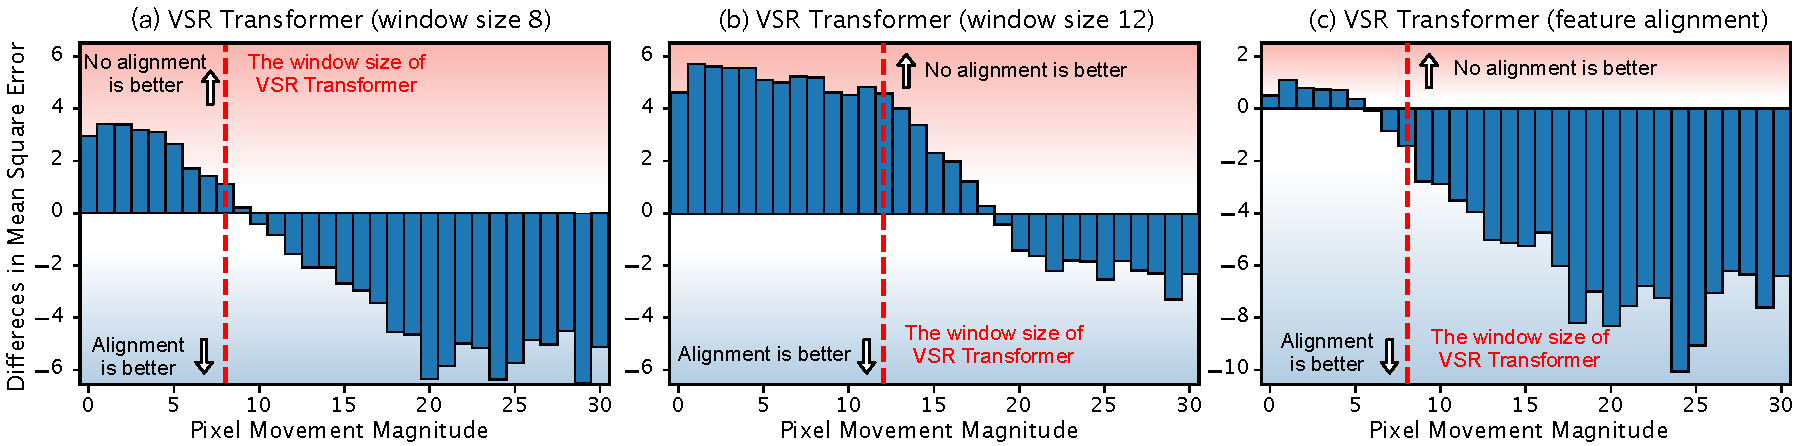
\includegraphics[width=\linewidth]{11.pdf}	
\caption{数据集像素运动分布情况统计}
\label{fig:fig11}
\end{figure}

综上,可以得到三个结论:第一个是 VSR Transformer可以在一定的范围内处理这种不对齐,而且是最好的,这种情况下加上Alignment 反而会损害它的性能;第二是处理的范围是与Transformer里面发挥全局处理的这个范围紧密相关;第三是对于超出这个范围的像素Alignment才是必要的。

\begin{figure*}[!tbp]
	\centering
	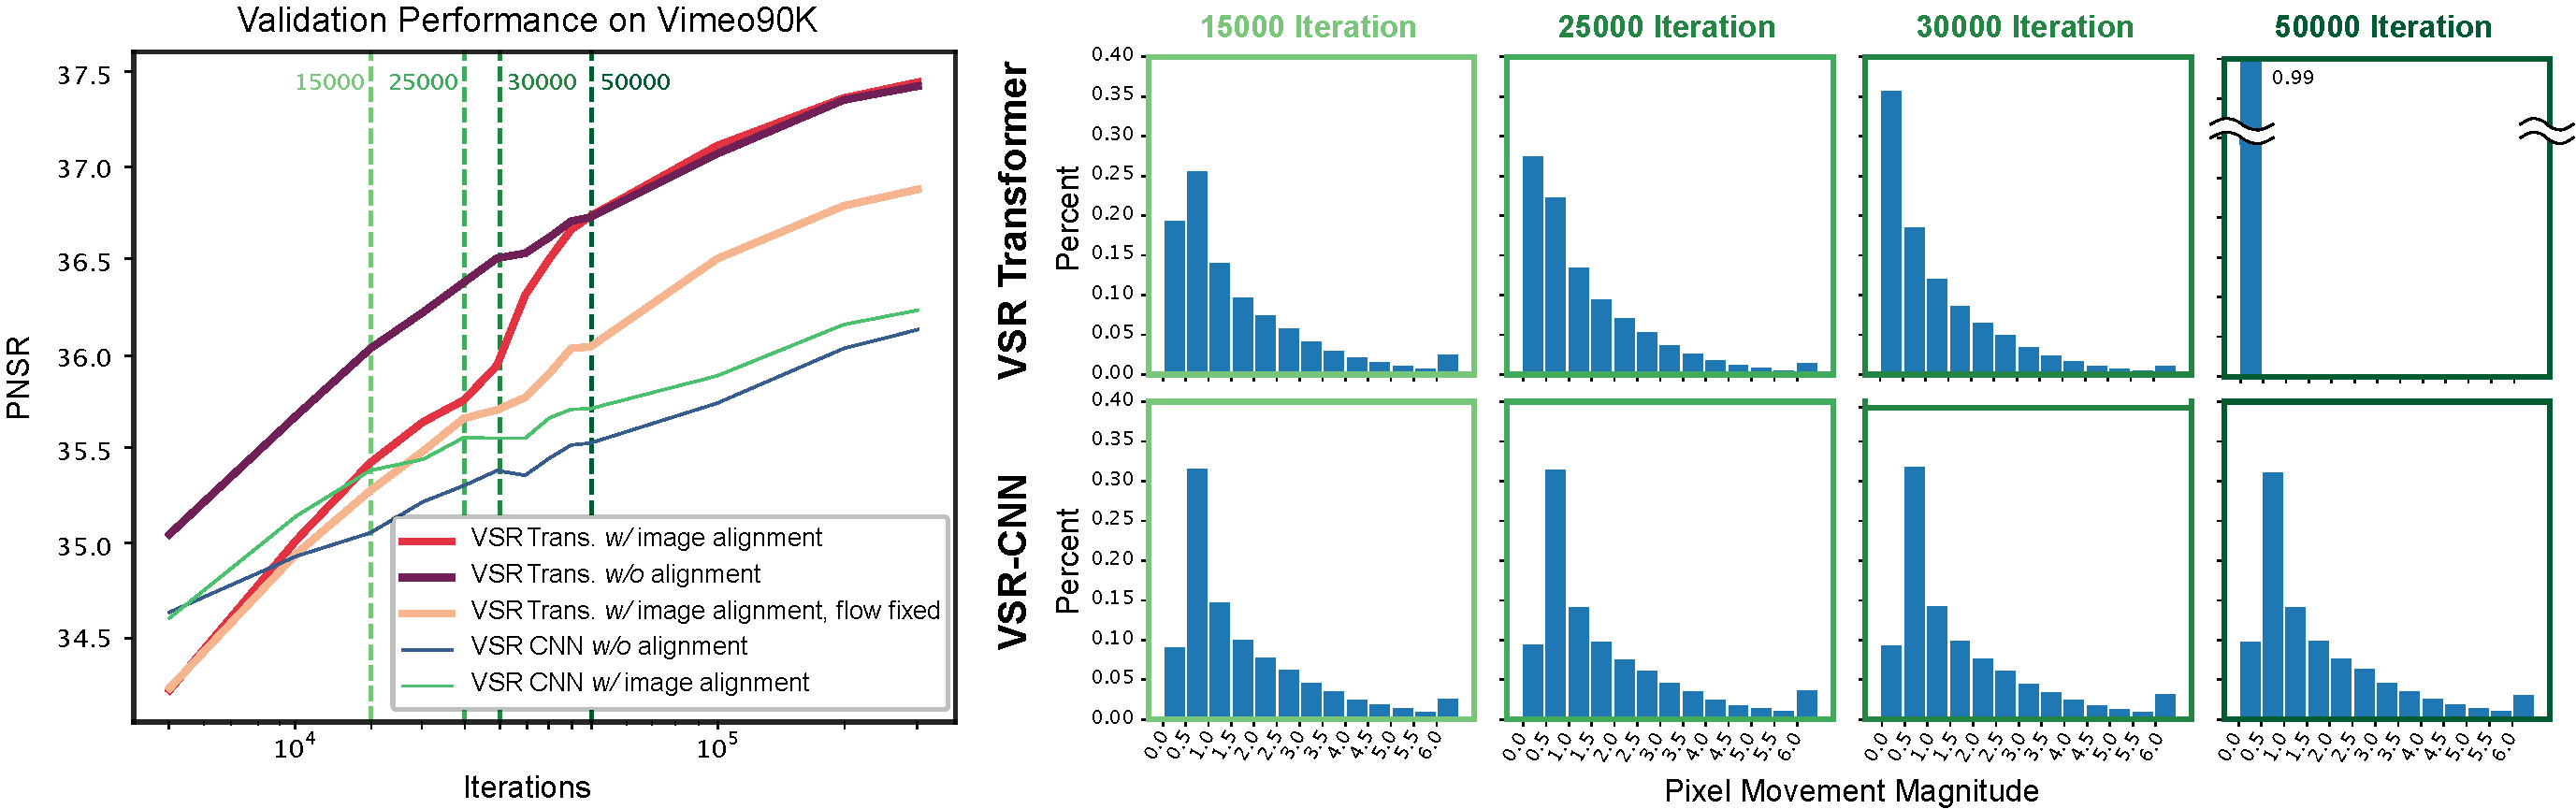
\includegraphics[width=\linewidth]{13.pdf}
	\caption{光流分布示意图}
	\label{fig:fig13}
\end{figure*}

\begin{table*}[!hb]
    \footnotesize
    \caption{Comparison of VSR Transformers with different alignment methods on the REDS4 dataset.}
    \centering
    \label{tab:3-10sliding}
    \vspace{1mm}
    \resizebox{\textwidth}{!}{
    \begin{tabular}{c|cccc|cc|cc|c|c}
        \toprule
        \multirow{2}{*}{\#} & \multicolumn{4}{c|}{Alignment Method} & \multicolumn{2}{c|}{Position} & \multicolumn{2}{c|}{Resampling} & Params. & REDS4\\
        & No Ali. & Img. Ali. & Feat. Ali. & FGDC & Img. & Feat. & BI & NN & (M) & PSNR / SSIM \\
        \midrule
        1 & $\checkmark$ & & & & & & & & 12.9 & 30.92 / 0.8759\\
        2 & & $\checkmark$ & & & $\checkmark$ & & $\checkmark$ & & 12.9 & 30.84 / 0.8752 \\
        3 & & & $\checkmark$ & & & $\checkmark$ & $\checkmark$ & & 14.8 & 31.06 / 0.8792 \\
        4 & & & $\checkmark$ & &  &$\checkmark$ & & $\checkmark$ & 14.8 & 31.11 / 0.8801 \\
        5 & & & & $\checkmark$ & & $\checkmark$ & & & 16.1 & 31.11 / 0.8804 \\
        \bottomrule
    \end{tabular}
    }
\label{tab:tab2}
\end{table*}

接下来再进一步的进行一个可视化或者可解释性的一个研究。为了进一步探究 Transformer 是否真的利用了多帧信息,利用Local Attribution Map高亮出对于处理选定的一小块区域那些非常有用的像素。例如在车牌上圈定一小块像素,用蓝色的线标识出了在中间帧对于这个车牌网络需要关注的位置,红色的区域就是在那一帧当中网络关注到的区域。对于配备了Image Alignment 的 CNN 而言,看到当车牌移开这个蓝色焦点的时候,网络的注意力其实是跟着车牌在走的,注意力红色区域它确实盯在了这个车牌的这个位置。再看不加Alignment的 Transformer,它也有相同的行为,当车牌进行移动的时候,可以发现它的注意力也是从蓝线的右边挪到了蓝线的左边,是跟随着这个物体在走的。也就是说Transformer在没有Alignment的时候他其实是做了一定的对齐的。相反,不加Alignment的CNN,无论车怎么移动,网络的关注点都只会聚焦在原来的位置。

\begin{figure*}[!tbp]
	\centering
	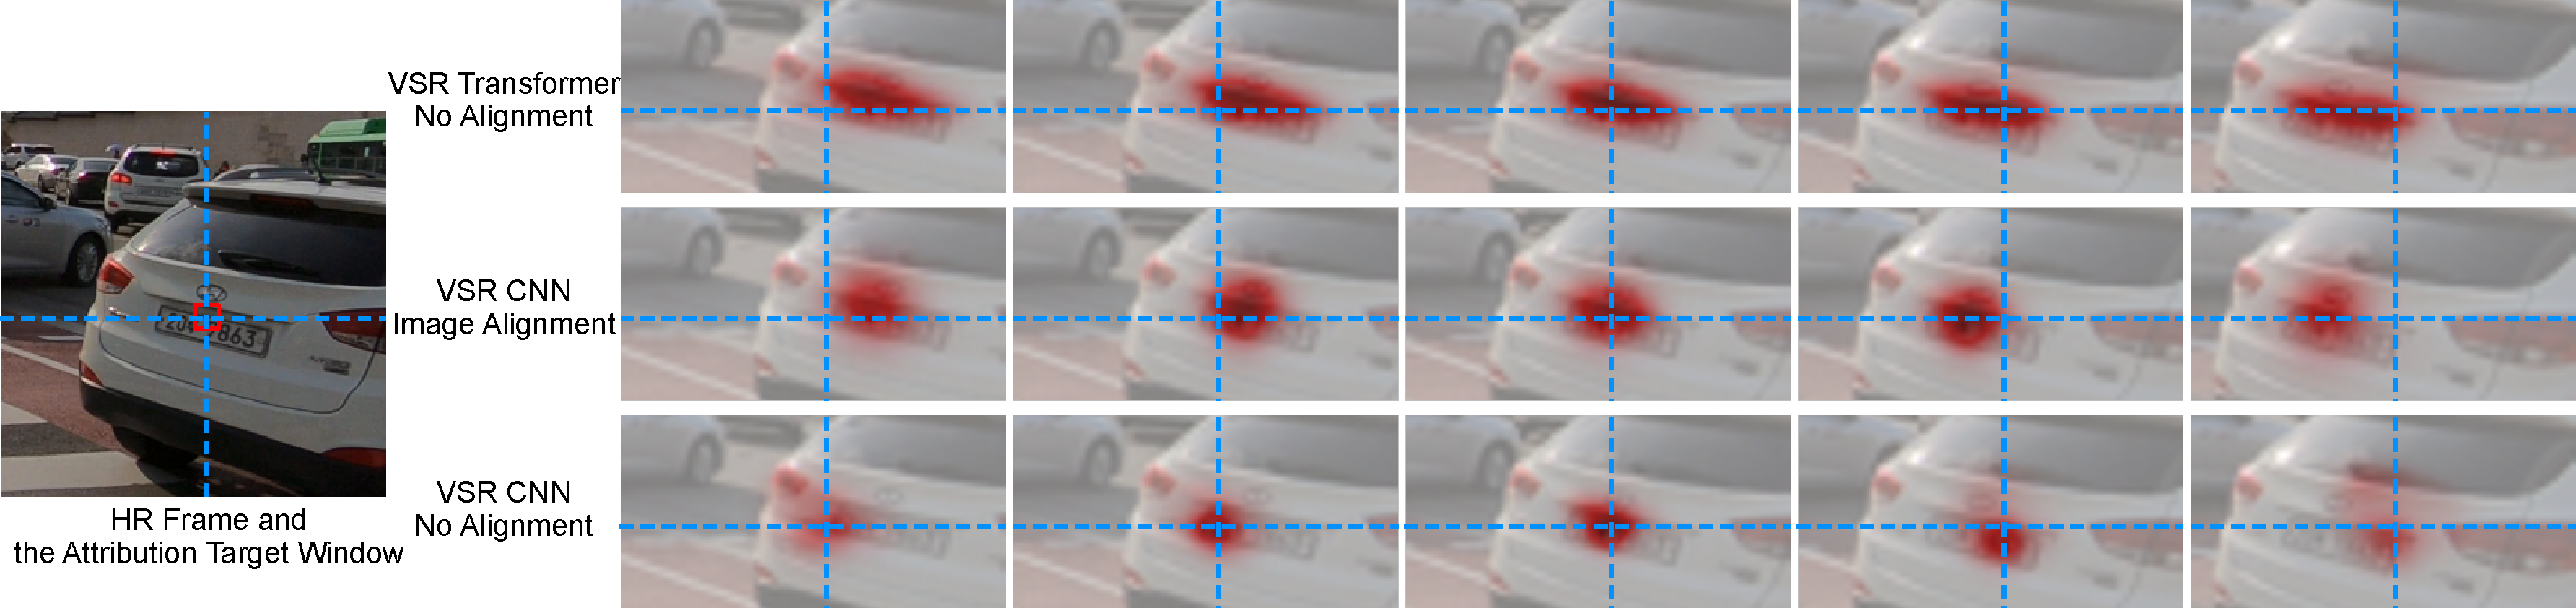
\includegraphics[width=\linewidth]{12.pdf}
	\caption{不同模型的归因结果}
	\label{fig:fig12}
\end{figure*}

\begin{figure*}[!tbp]
	\centering
	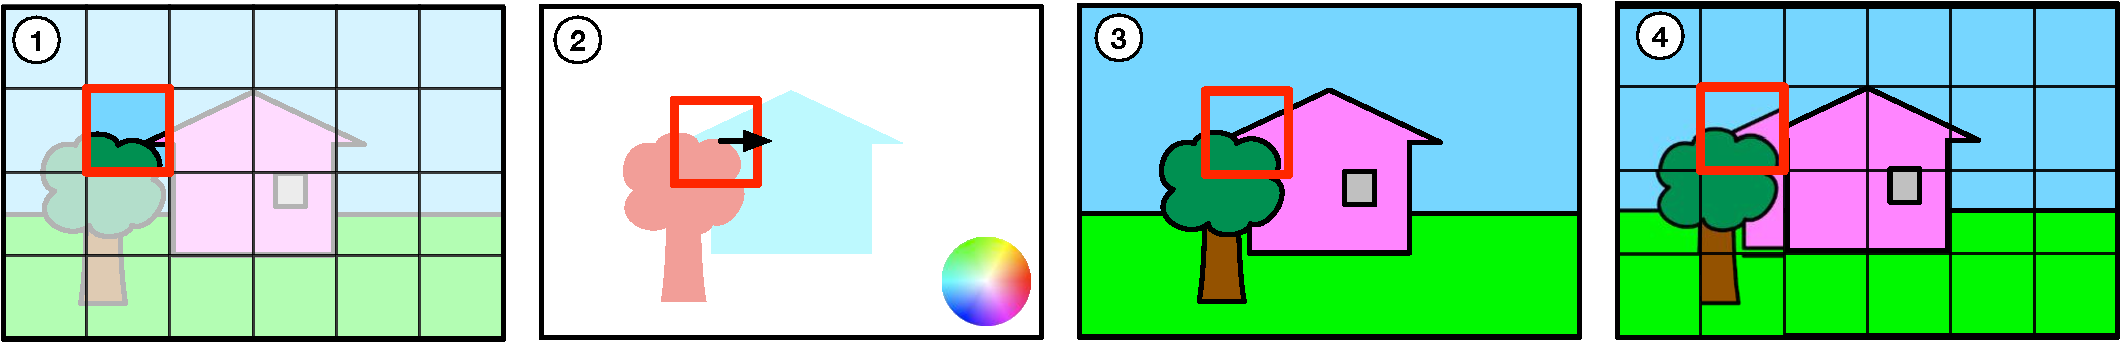
\includegraphics[width=\linewidth]{14.pdf}
	\caption{Patch Alignment: 根据 Transformer 的窗口划分将输入帧划分为 patch,计算每个 patch 的平均运动矢量,在支持帧中找到相应的 patch,并将整个支持 patch 移动到它们相应的位置}
	\label{fig:fig14}
\end{figure*}

对于第二个问题,刚才已经提到了在一定范围内用了alignment 反而会降低它的性能。从实验结果 \textbf{表 \ref{tab:tab1}} 可以看到,就是在 Image Alignment 里,对光流网络进行 Finetune 要比把预测光流的网络固定住要好,因为此时这个网络学习优化的是 VSR 的光流。第二个发现是使用Image Alignment 并 Finetune在Vimeo90K上是37.44,而同样的网络去掉Alignment是37.43非常接近的一个成绩。而在REDS数据集上,后者更是提升了0.13个db。



如 \textbf{图 \ref{fig:fig13}} 所示,最上面的线是是不加 Alignment,红色的线是 Fine Tune 光流网络的线,黄色的线是不Finetune, 可以看到光流固定住之后它的效果肯定就一直和不使用Alignment的保持一定的距离。而红色的线一开始因为初值相同,和 Fix flow的结果是比较接近的,然后随着训练展示出了一点优势,到中间的时候立马追上了不使用Alignment的方法。从预测出来的光流分布可以看到,在25000和30000个iteration的时候分布开始往这个零的方向移动,性能追上来之后,所有的光流都是零。这表明网络认为你虽然给了我这个对齐的模块,但是我发现我不使用你这个对齐模块才是最好的。为了验证说这个东西确实是Transformer特有的,还在CNN上面做了测试,取得了完全不同的结果。


如 \textbf{表 \ref{tab:tab2}} 所示,通过实验发现,造成这个差距的原因主要有两方面,一是预测的光流是有噪声的、不平滑的,这会造成 Warping 的不准确。例如,相邻的两个像素是以不同的光流进行Warping 的,一个往左移动挪了一个像素,另外一个往左移动了0.5个像素,也就是说可能原来这个像素是黑的,另一个像素是白的,Warping 之后移动一个像素位置的像素还是黑色的,移动了0.5个像素位置的像素经过插值不再是白色的,而变成灰色了。在这个过程中,低分辨率的模式中一黑一白经过变成了一黑一灰,即亚像素的信息被改变了,这个改变是一种完全随机的改变,从而减少和伤害了亚像素信息的质量,因而会导致性能的下降。二是在Warping的过程中可能需要重采样,也会引入新的像素值,进而引入新的这个信息损失。在Feature Alignment方法中,简单地把重采样过程从原来广泛使用的双线性采样变成最近邻采样,即Warping前后像素的值是不会改变的,可以看到模型的性能就能达到现在最先进的Flow Guided Deformable Convolution 的一个效果。侧面证明了一部分信息损失是由Eesampling和不准确的光流造成的。

\begin{table}[!ht]
\caption{The Ablation study of Patch Align- ment. We study the effect of different re- sampling methods (BI and NN) and differ- ent alignment positions (image space and feature space).}
    \centering
    \resizebox{0.5\textwidth}{!}{
        \begin{tabular}{c|cc|cc|cc}
        \toprule
        \multirow{2}{*}{Method} & \multicolumn{2}{c|}{Position} & \multicolumn{2}{c|}{Resampling} & \multicolumn{2}{c}{REDS4}\\
         & Img. & Feat. & BI & NN & PSNR & SSIM \\
        \midrule
        \multirow{3}{*}{\shortstack{Patch\\Alignment}} & $\checkmark$ & & & $\checkmark$ & 31.11 & 0.8800 \\
         & & $\checkmark$ & $\checkmark$ & & 31.00 & 0.8781 \\
         & & $\checkmark$ & & $\checkmark$ & 31.17 & 0.8810 \\
        \bottomrule
    \end{tabular}
    }
    \hfill
    % \resizebox{0.38\textwidth}{!}{
    \label{tab:tab3}
\end{table}

至此得到了两个核心的结论:第一个就是Transformer确实可以直接使用没有经过对齐的信息,第二个是现有的这些对齐方法实际上是损失了VSR Transformer 的性能。

而为了设计一个更好的VSR模型,可以简单地扩大Attention Window Size,但这样做会带来巨大的计算开销。因此,作者提出了一个新的对齐方法Patch Alignment。由于光流是不准确的,那么就只用这个大概的这么一个光流,为了不让低分辨率的模式有任何的破坏,直接利用光流均值对整个 Patch进行大概的移动,如 \textbf{图 \ref{fig:fig14}} 所示。

\begin{figure*}[!tbp]
	\centering
	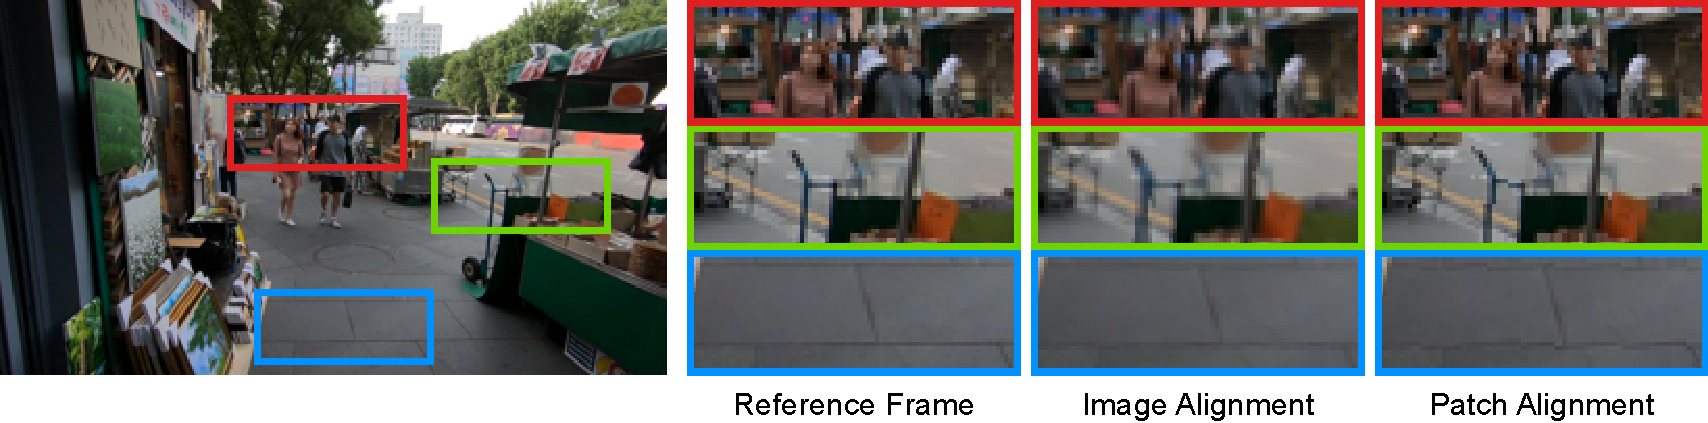
\includegraphics[width=\linewidth]{15.pdf}
	\caption{Image Alignment 和 Patch Alignment可视化结果}
	\label{fig:fig15}
\end{figure*}

再看一下可视化的结果,如 \textbf{图 \ref{fig:fig15}} 所示,第二列是使用Image Alignment的配上双线性插值的重采样,可以看到人脸上非常细小的信息都被模糊掉了,地砖两个像素之间的关系也被破坏掉了。而本文的 Patch Alignment,可以看到这个把手非常的锐利,虽然它有一点点的不对齐,但是这种像素的错位不会带来什么影响,反而只要一个Patch里面的信息不要破坏它就已经是非常好了。

\section{实验}
\label{sec:experiment}

\begin{table*}[t]
\footnotesize
\caption{ Quantitative comparison of different VSR methods. The results marked with ∗ achieve similar performance as no alignment. This is due to the vanishing of optical flow in this experiment.}
\centering
\resizebox{\textwidth}{!}{
    \begin{tabular}{c|l|ll|cc|cc}
        \toprule
        Exp. &
        \multirow{2}{*}{Method} &
        \multirow{2}{*}{Alignment} & \multirow{2}{*}{Remark} & \multicolumn{2}{c|}{Vimeo90K-T} & \multicolumn{2}{c}{REDS4}\\
        Index & & & & PSNR & SSIM & PSNR & SSIM\\
        \midrule
        1 & VSR-CNN & Image alignment & Finetune flow & 36.13 & 0.9342 & 29.81 & 0.8541\\
        2 & VSR-CNN & No alignment &  & 36.24 & 0.9359 & 28.95 &  0.8280\\
        3 & VSR Transformer & Image alignment & Fix flow  & 36.87 & 0.9429 & 30.25 & 0.8637\\
        4 & VSR Transformer & Image alignment & Finetune flow & 37.44$^*$ & 0.9472$^*$ & 30.43 &  0.8677\\
        5 & VSR Transformer & Feature alignment & Finetune flow & 37.36 & 0.9468 & 30.74 & 0.8740\\
        6 & VSR Transformer & No alignment & Window size 8 & 37.43 & 0.9470 & 30.56 & 0.8696\\
        7 & VSR Transformer & No alignment & Window size 16 & 37.46 & 0.9474 & 30.81 & 0.8745\\
        \bottomrule
    \end{tabular}}
    \label{tab:tab1}
\end{table*}

可以看到,在Image上面使用Patch Alignment就已经可以达到现在最好的一个效果,而且节省了将近2~3兆的参数量。在Feature的层面进行Patch Alignment,达到31.17。

在主流Benchmark上的结果证明了该方法是有效的,在Recurrent只使用六帧进行训练时,能拿到31.88的成绩,使用16帧进行训练时,在REDS上能拿到32.72的成绩。

一些可视化的结果也证明了,例如车牌低分辨率的版本几乎什么都不剩了,但是结合近邻帧可以对它进行一个非常好的重建。可以看到本文的方法是可以把大楼的条纹和窗户给重建出来的。

\begin{figure*}[!htbp]
	\centering
	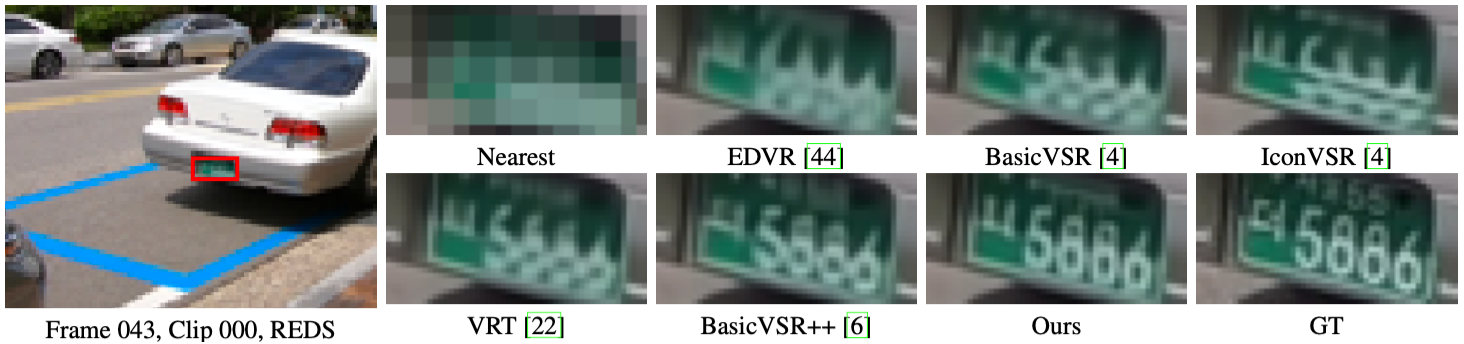
\includegraphics[width=\linewidth]{17.png}
	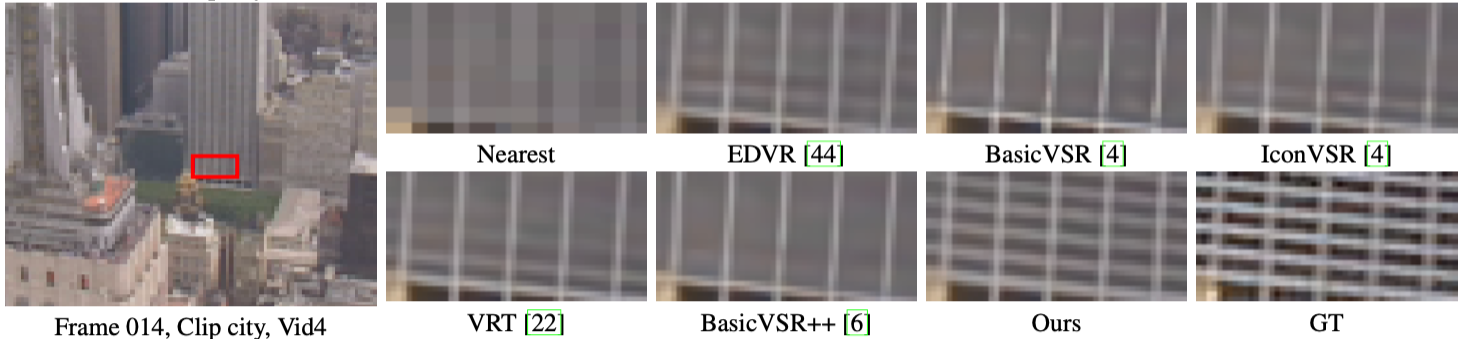
\includegraphics[width=\linewidth]{18.png}
	\caption{VSR (×4) 可视化结果}
\end{figure*}
\section{总结}
\label{sec:conclusion}

传统数字图像处理方法使用成熟的技术处理问题,如特征描述子(SIFT、SUR、BRIEF 等)。在深度学习兴起前,图像分类等任务需要用到特征提取步骤,特征即图像中``有趣''、描述性或信息性的小图像块。这一步可能涉及多种数字图像处理算法,如边缘检测、角点检测或阈值分割算法。从图像中提取出足够多的特征后,这些特征可形成每个目标类别的定义(即``词袋'')。部署阶段中,在其他图像中搜索这些定义。如果在一张图像中找到了另一张图像词袋中的绝大多数特征,则该图像也包含同样的目标(如椅子、马等)。传统方法的缺陷是从每张图像中选择重要特征是必要步骤。而随着类别数量的增加,特征提取变得越来越麻烦。要确定哪些特征最能描述不同的目标类别,取决于研究人员的判断和长期试错。此外,每个特征定义还需要处理大量参数,所有参数必须由人来进行调整。

而深度学习的快速发展和设备能力的改善(如算力、内存容量、能耗、图像传感器分辨率和光学器件)提升了视觉应用的性能和成本效益,并进一步加快了此类应用的扩展。与传统方法相比,深度学习可以帮助 研究人员在图像分类、语义分割和目标检测等任务上获得更高的准确率。由于深度学习所用的神经网络是训练得到而非编程得到,因此使用该方法的应用所需的专家分析和微调较少,且能够处理目前系统中的海量可用视频数据。深度学习引入了端到端学习的概念,即向计算机提供的图像数据集中的每张图像均已标注目标类别。因而深度学习模型基于给定数据``训练''得到,其中神经网络发现图像类别中的底层模式,并自动提取出对于目标类别最具描述性和最显著的特征。

但这并不意味着传统方法的没落,在本文的调研和分析中,可以看到即使在深度学习大放异彩的时代,仍在一定程度上依赖于传统方法的使用,甚至从中获得理论指导或思路启迪,如正交变换、高斯滤波等。传统数字图像处理方法和深度学习方法之间存在一定的权衡。传统方法成熟、透明,且为性能和能效进行过优化;深度学习提供更好的准确率和通用性,但消耗的计算资源也更大。混合方法结合传统方法和深度学习,兼具这两种方法的优点,更加适用于需要快速实现的高性能系统。

% Can use something like this to put references on a page
% by themselves when using endfloat and the captionsoff option.
\ifCLASSOPTIONcaptionsoff
  \newpage
\fi



%{\small
%\bibliographystyle{IEEEtran}
%\bibliography{reference/egbib}
%}

% that's all folks
\end{sloppypar}
\end{document}


